% =====================================================================
%  MATH 55 -- Lecture Notes & Reviewer No. 7
%  Vector Calculus: vector fields, gradient fields, conservative fields
%  Build: latexmk -pdf -outdir=build lecture-notes-03.tex
% =====================================================================
\documentclass[11pt,a4paper]{article}

\newcommand{\NotesNumber}{7}
\newcommand{\NotesKind}{Lecture Notes \& Reviewer No.~7}
\newcommand{\NotesShortTitle}{Vector Calculus}
\newcommand{\NotesPdfTitle}{MATH 55 Lecture Notes 7: Vector Calculus}
% =====================================================================
%  MATH 55 -- Shared preamble for the Second Long Exam reviewers
%  Reproduces the look of "Lecture Notes 01" (Lecture Notes & Reviewer
%  No. 5): Latin Modern, small-caps running heads, ruled chapter titles,
%  amsthm environments numbered within chapters, framed strategy boxes.
%
%  Each document defines, BEFORE \input-ing this file:
%     \NotesNumber      e.g. 6
%     \NotesKind        e.g. Lecture Notes \& Reviewer No.~6
%     \NotesShortTitle  e.g. Directional Derivatives and Gradient
%     \NotesPdfTitle    plain-text title for the PDF metadata
% =====================================================================

% ---------- Fonts and encoding --------------------------------------
\usepackage[T1]{fontenc}
\usepackage[utf8]{inputenc}
\usepackage{lmodern}
\usepackage{microtype}

% ---------- Page geometry -------------------------------------------
\usepackage[a4paper,top=1in,bottom=1in,left=1.05in,right=1.05in,
            headheight=15pt,footskip=30pt]{geometry}
\setlength{\parindent}{0pt}
\setlength{\parskip}{6pt plus 2pt minus 1pt}

% ---------- Mathematics ---------------------------------------------
\usepackage{amsmath,amssymb,amsthm,mathtools}
\usepackage{bm}

% ---------- Graphics, tables, lists ---------------------------------
\usepackage{graphicx}
\usepackage[dvipsnames]{xcolor}
\usepackage{tikz}
\usetikzlibrary{arrows.meta,calc,angles,quotes,positioning}
\usepackage{pgfplots}
\pgfplotsset{compat=1.17}
\usepackage{booktabs,array,tabularx,multirow}
\usepackage{caption}
\usepackage{subcaption}
\captionsetup{font=small,labelfont=bf,width=0.92\linewidth}
\usepackage{enumitem}
\setlist{itemsep=2pt,topsep=4pt}
\usepackage{float}
\usepackage[most]{tcolorbox}

% ---------- Headings --------------------------------------------------
\usepackage{titlesec}
% "Chapter N" over a ruled small-caps title, each on a new page
\titleformat{\section}[display]
  {\normalfont\centering}
  {\large\scshape Chapter \thesection}
  {8pt}
  {\titlerule\vspace{10pt}\LARGE\scshape}
  [\vspace{4pt}\titlerule]
\titlespacing*{\section}{0pt}{0pt}{22pt}
\newcommand{\sectionbreak}{\clearpage}
\titleformat{\subsection}{\normalfont\large\bfseries}{\thesubsection}{1em}{}
\titleformat{\subsubsection}{\normalfont\normalsize\bfseries}{\thesubsubsection}{1em}{}
\setcounter{tocdepth}{2}

% Appendices are titled "Appendix A" instead of "Chapter A"
\newcommand{\startappendix}{%
  \appendix
  \titleformat{\section}[display]
    {\normalfont\centering}
    {\large\scshape Appendix \thesection}
    {8pt}
    {\titlerule\vspace{10pt}\LARGE\scshape}
    [\vspace{4pt}\titlerule]%
}

% ---------- Running heads and feet ----------------------------------
\usepackage{fancyhdr}
\newcommand{\NotesAuthor}{Juevesano, D.}
\fancypagestyle{m55}{%
  \fancyhf{}%
  \fancyhead[L]{\small\textsc{\NotesKind}}%
  \fancyhead[R]{\small\textsc{Math 55 -- \NotesShortTitle}}%
  \fancyfoot[L]{\small\NotesAuthor\ 2026 ALL RIGHTS RESERVED. Not for redistribution.}%
  \fancyfoot[R]{\small\thepage}%
  \renewcommand{\headrulewidth}{0.4pt}%
  \renewcommand{\footrulewidth}{0.4pt}%
}
% chapter-opening pages use "plain": keep the same head/foot there too
\fancypagestyle{plain}{%
  \fancyhf{}%
  \fancyhead[L]{\small\textsc{\NotesKind}}%
  \fancyhead[R]{\small\textsc{Math 55 -- \NotesShortTitle}}%
  \fancyfoot[L]{\small\NotesAuthor\ 2026 ALL RIGHTS RESERVED. Not for redistribution.}%
  \fancyfoot[R]{\small\thepage}%
  \renewcommand{\headrulewidth}{0.4pt}%
  \renewcommand{\footrulewidth}{0.4pt}%
}
\pagestyle{m55}

% ---------- Theorem-like environments --------------------------------
\theoremstyle{definition}
\newtheorem{definition}{Definition}[section]
\newtheorem{example}[definition]{Example}
\newtheorem{problem}[definition]{Problem}
\newtheorem{exercise}[definition]{Exercise}
\theoremstyle{plain}
\newtheorem{theorem}[definition]{Theorem}
\newtheorem{proposition}[definition]{Proposition}
\newtheorem{corollary}[definition]{Corollary}
\newtheorem{lemma}[definition]{Lemma}
\theoremstyle{remark}
\newtheorem{remark}[definition]{Remark}
\newtheorem{warning}[definition]{Warning}

\newenvironment{solution}{\begin{proof}[Solution]}{\end{proof}}
% bold step labels inside solutions, e.g. \step{1}{Partial derivatives.}
\newcommand{\step}[2]{\par\smallskip\noindent\textbf{Step #1: #2}\ }
\newcommand{\stepx}[1]{\par\smallskip\noindent\textbf{#1}\ }
\newcommand{\checkok}{\ \checkmark}

% ---------- Boxes -----------------------------------------------------
% Framed "Strategy" box (as on p. 7 of Lecture Notes 01)
\newtcolorbox{strategy}[1]{%
  enhanced,breakable,colback=white,colframe=black!75,boxrule=0.6pt,
  sharp corners,left=10pt,right=10pt,top=8pt,bottom=8pt,
  before upper={\textbf{#1}\par\smallskip}}
% Highlighted key-result box
\newtcolorbox{keybox}[1]{%
  enhanced,breakable,colback=black!3,colframe=black!75,boxrule=0.6pt,
  sharp corners,left=10pt,right=10pt,top=8pt,bottom=8pt,
  before upper={\textbf{#1}\par\smallskip}}

% "Alternative method" box: a quicker route shown AFTER the full solution
\newtcolorbox{altmethod}{%
  enhanced,breakable,colback=white,colframe=black!45,boxrule=0.5pt,
  sharp corners,left=10pt,right=10pt,top=6pt,bottom=6pt,
  before upper={\textbf{Alternative method (optional).}\ }}
% Boxed concluding sentence of a solution
\newcommand{\finalans}[1]{\par\smallskip\noindent\textbf{Final answer.}\ #1}

% ---------- Notation --------------------------------------------------
\newcommand{\R}{\mathbb{R}}
\newcommand{\vb}[1]{\mathbf{#1}}
\newcommand{\vi}{\mathbf{i}}
\newcommand{\vj}{\mathbf{j}}
\newcommand{\vk}{\mathbf{k}}
\newcommand{\vu}{\mathbf{u}}
\newcommand{\vv}{\mathbf{v}}
\newcommand{\vr}{\mathbf{r}}
\newcommand{\vx}{\mathbf{x}}
\newcommand{\vF}{\mathbf{F}}
\newcommand{\vT}{\mathbf{T}}
\newcommand{\vN}{\mathbf{N}}
\newcommand{\vB}{\mathbf{B}}
\newcommand{\vzero}{\mathbf{0}}
\newcommand{\ip}[1]{\left\langle #1 \right\rangle}
\DeclarePairedDelimiter{\norm}{\lVert}{\rVert}
\DeclarePairedDelimiter{\abs}{\lvert}{\rvert}
\newcommand{\dd}{\mathrm{d}}
\newcommand{\Du}{D_{\mathbf{u}}}
\newcommand{\grad}{\nabla}
\newcommand{\pd}[2]{\frac{\partial #1}{\partial #2}}
\newcommand{\vecPQ}{\overrightarrow{PQ}}
\newcommand{\eval}[1]{\Big|_{#1}}

% ---------- Interactive links (underlined, like Lecture Notes 01) ----
\newcommand{\extlink}[2]{\href{#1}{\underline{#2}}}
\newcommand{\interactive}[2]{%
  \par\noindent\textit{Interactive:} \extlink{#1}{#2}\ }
\newcommand{\desmosTD}{https://www.desmos.com/3d}
\newcommand{\desmosTwoD}{https://www.desmos.com/calculator}

% ---------- Hyperref (load last) -------------------------------------
\usepackage[hidelinks]{hyperref}
\hypersetup{pdfauthor={Juevesano, D.},pdftitle={\NotesPdfTitle}}

% ---------- Title page -----------------------------------------------
% \makenotestitle{Title}{Subtitle}{Line under "No. N"}{About text}
\newcommand{\makenotestitle}[4]{%
  \begingroup
    \thispagestyle{plain}
    \centering
    \vspace*{1.6cm}
    {\large\scshape University of the Philippines Cebu\par
     Mathematics Program\par}
    \vspace{1.6cm}
    \rule{\linewidth}{0.5pt}\par\vspace{0.8cm}
    {\Huge\scshape #1\par}
    \vspace{0.5cm}
    {\large #2\par}
    \vspace{0.8cm}\rule{\linewidth}{0.5pt}\par
    \vspace{1.4cm}
    {\large\scshape \NotesKind\par}
    \vspace{0.4cm}
    {#3\par}
    \vfill
    \begin{minipage}{0.84\linewidth}
      \small\raggedright #4
    \end{minipage}
    \vfill
    {\NotesAuthor\quad 2026\par}
    \vspace{0.6cm}
  \clearpage
  \endgroup
}

% The table of contents is a starred \section, so it automatically gets
% the centred, ruled small-caps title used for chapters.

\graphicspath{{figures/}}

\begin{document}
\pagenumbering{roman}

\makenotestitle{Vector Calculus}
  {Vector Fields, Gradient Fields, Conservative Fields and Potential Functions}
  {MATH 55: Elementary Analysis III -- Second Long Examination}
  {\textbf{About these notes.} These notes expand the course slides
   \emph{M55 -- 7 Vector Calculus} (as of November~5) into a complete written
   treatment. Chapters~2--4 reproduce every definition, theorem, example and
   exercise of the slides (vector fields, gradient fields, conservative
   fields, the component test and the three-step method for potential
   functions) with full solutions, including Exercises~1--4.
   Chapter~5 is a large bank of exam-style problems with complete solutions.
   \emph{Scope:} line integrals and the Fundamental Theorem for Line
   Integrals (Parts IV--VI of the slide overview) are \emph{not} covered by
   this exam and are deliberately left out.\par\medskip
   \textbf{Prerequisites.} Gradients (Lecture Notes No.~6) and vector
   functions, derivatives and arc length (Lecture Notes No.~5). Every
   numerical answer has been checked with a computer algebra system.}

\tableofcontents
\clearpage
\pagenumbering{arabic}

% =====================================================================
\section{Preliminaries}\label{ch:prelim}
% =====================================================================

Vector calculus combines the two objects studied in the previous reviewers:
\emph{vector functions} $\vr(t)$, which describe curves (No.~5), and
\emph{gradients} $\grad f$, which describe how a scalar function changes
(No.~6). This chapter recalls exactly the facts that will be used.

\subsection{Gradients}

For $f(x,y)$ and $f(x,y,z)$,
\[
  \grad f=\ip{f_x,f_y}=f_x\vi+f_y\vj,\qquad
  \grad f=\ip{f_x,f_y,f_z}=f_x\vi+f_y\vj+f_z\vk .
\]
$\grad f$ points in the direction of fastest increase of $f$, has length equal
to that maximal rate, and is perpendicular to the level curves (surfaces) of
$f$.

\subsection{Curves, tangent vectors and arc length}

A (smooth) curve $C$ is described by a vector function
\[
  \vr(t)=\ip{x(t),y(t)}\quad\text{or}\quad\vr(t)=\ip{x(t),y(t),z(t)},\qquad a\le t\le b,
\]
with $\vr\,'(t)$ continuous and never $\vzero$. As $t$ increases from $a$ to $b$
the point moves from the \emph{initial point} $\vr(a)$ to the \emph{terminal
point} $\vr(b)$; this gives $C$ an \emph{orientation}.
\begin{itemize}
  \item $\vr\,'(t)$ is tangent to $C$ and points in the direction of motion.
  \item The \emph{speed} is $\norm{\vr\,'(t)}$, and the arc length element is
        $\dd s=\norm{\vr\,'(t)}\,\dd t$, so the length of $C$ is
        $L=\int_a^b\norm{\vr\,'(t)}\,\dd t$.
\end{itemize}

\begin{strategy}{Standard parametrizations (memorize).}
\begin{itemize}
  \item Segment from $P_0$ to $P_1$: $\;\vr(t)=(1-t)\vr_0+t\vr_1=\vr_0+t(\vr_1-\vr_0)$, $0\le t\le1$.
  \item Circle $x^2+y^2=R^2$, counterclockwise: $\;\vr(t)=\ip{R\cos t,R\sin t}$, $0\le t\le2\pi$.
  \item Graph $y=g(x)$, $a\le x\le b$: $\;\vr(t)=\ip{t,g(t)}$, $a\le t\le b$.
  \item Graph $x=h(y)$: $\;\vr(t)=\ip{h(t),t}$.
  \item Helix: $\;\vr(t)=\ip{\cos t,\sin t,t}$.
\end{itemize}
\end{strategy}

\begin{example}\label{ex:prelim-seg}
Parametrize the segment from $(2,0,0)$ to $(3,4,5)$ and find its length.
\end{example}
\begin{solution}
$\vr(t)=\ip{2,0,0}+t\ip{1,4,5}=\ip{2+t,\,4t,\,5t}$, $0\le t\le1$. Then
$\vr\,'(t)=\ip{1,4,5}$, $\norm{\vr\,'(t)}=\sqrt{42}$, and $L=\int_0^1\sqrt{42}\,\dd t=\sqrt{42}$
(which is, of course, the distance between the two points).
\end{solution}

\subsection{Equality of mixed partial derivatives}

The test for conservative vector fields in Chapter~\ref{ch:conservative} rests
on the following theorem.

\begin{theorem}[Clairaut]\label{thm:clairaut}
If $f$ is defined on an open disk containing $(a,b)$ and $f_{xy}$, $f_{yx}$ are
both continuous there, then $f_{xy}(a,b)=f_{yx}(a,b)$. The same holds for
functions of three variables and any pair of variables.
\end{theorem}

\begin{example}\label{ex:clairaut}
Verify Clairaut's theorem for $f(x,y)=x^3y^2+e^{xy}$.
\end{example}
\begin{solution}
$f_x=3x^2y^2+ye^{xy}$, so $f_{xy}=(f_x)_y=6x^2y+e^{xy}+xye^{xy}$.\\
$f_y=2x^3y+xe^{xy}$, so $f_{yx}=(f_y)_x=6x^2y+e^{xy}+xye^{xy}$. They agree.\checkok
\end{solution}

\subsection{Partial integration}

To recover a function from one of its partial derivatives we integrate with
respect to one variable while holding the others fixed. Because anything that
does not depend on the integration variable differentiates to zero, the
``constant of integration'' is an arbitrary \emph{function of the other
variables}.

\begin{example}\label{ex:partial-int}
Find all functions $f(x,y)$ with $f_x=2xy+y^3$.
\end{example}
\begin{solution}
Integrate with respect to $x$, treating $y$ as a constant:
\[
  f(x,y)=\int(2xy+y^3)\,\dd x=x^2y+xy^3+g(y),
\]
where $g$ is an arbitrary differentiable function of $y$ alone. Check:
$\pd{}{x}\big(x^2y+xy^3+g(y)\big)=2xy+y^3+0$.\checkok
\end{solution}

\begin{warning}
Writing ``$+C$'' instead of ``$+g(y)$'' here is a serious error: it throws
away information that is needed in the next step of the potential-function
method (Section~\ref{sec:potential}).
\end{warning}

\subsection{Types of regions}

\begin{itemize}
  \item A region $D$ is \emph{open} if around each of its points there is a
        small disk (ball) contained in $D$; e.g. an open disk, the whole plane,
        the plane minus a point.
  \item $D$ is \emph{connected} if any two points of $D$ can be joined by a
        path lying in $D$.
  \item A connected region in the plane is \emph{simply connected} if every
        simple closed curve in $D$ encloses only points of $D$; informally,
        $D$ has no holes. A disk, a half-plane and $\R^2$ are simply connected;
        an annulus and the punctured plane $\R^2\setminus\{(0,0)\}$ are not.
        (In space, $\R^3$ with a single point removed \emph{is} simply
        connected, while $\R^3$ minus a whole line is not.)
\end{itemize}

\begin{figure}[H]
\centering
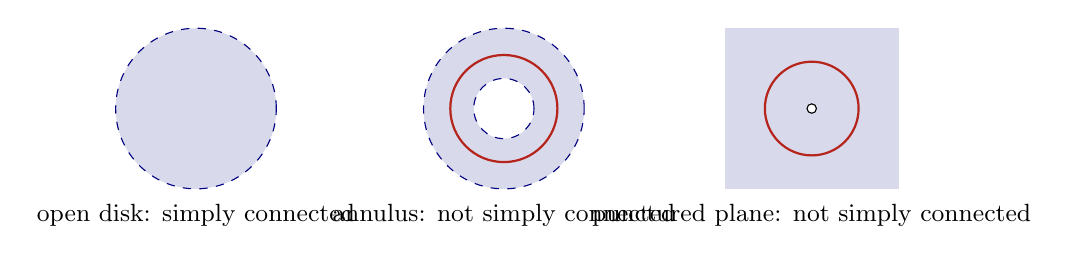
\begin{tikzpicture}[scale=0.85]
  \begin{scope}
    \fill[NavyBlue!15] (0,0) circle (1.2);
    \draw[NavyBlue,dashed] (0,0) circle (1.2);
    \node at (0,-1.6) {\small open disk: simply connected};
  \end{scope}
  \begin{scope}[xshift=4.6cm]
    \fill[NavyBlue!15, even odd rule] (0,0) circle (1.2) (0,0) circle (0.45);
    \draw[NavyBlue,dashed] (0,0) circle (1.2);
    \draw[NavyBlue,dashed] (0,0) circle (0.45);
    \draw[BrickRed,thick] (0,0) circle (0.8);
    \node at (0,-1.6) {\small annulus: not simply connected};
  \end{scope}
  \begin{scope}[xshift=9.2cm]
    \fill[NavyBlue!15] (-1.3,-1.2) rectangle (1.3,1.2);
    \filldraw[fill=white,draw=black] (0,0) circle (2pt);
    \draw[BrickRed,thick] (0,0) circle (0.7);
    \node at (0,-1.6) {\small punctured plane: not simply connected};
  \end{scope}
\end{tikzpicture}
\caption{The red loops in the middle and right pictures surround points that
are not in the region; they cannot be shrunk to a point inside the region.}
\label{fig:regions}
\end{figure}

These words matter because the component test for conservative fields
(Theorems~\ref{thm:test2} and~\ref{thm:test3}) is only guaranteed on
simply connected regions, such as the open disks and open balls named in the
slides; see Section~\ref{sec:caveat}.

% =====================================================================
\section{Vector Fields}\label{ch:fields}
% =====================================================================

A \emph{vector field} is a function whose domain is a set of points in $\R^2$
(or $\R^3$) and whose range is a set of vectors in $\R^2$ (or $\R^3$) (Slides).
Think of the wind: at every point of a map there is a wind velocity, a vector
with a direction and a strength.

\subsection{Definitions}

\begin{definition}[Vector field on $\R^2$; Slides, Definition 1]\label{def:vf2}
Let $D$ be a set in $\R^2$ (a plane region). A \emph{vector field on $\R^2$} is a
function $\vF$ that assigns to each point $(x,y)$ in $D$ a two-dimensional
vector $\vF(x,y)$:
\[
  \vF(x,y)=\ip{M(x,y),\,N(x,y)}=M(x,y)\,\vi+N(x,y)\,\vj .
\]
\end{definition}

\begin{definition}[Vector field on $\R^3$; Slides, Definition 2]\label{def:vf3}
Let $E$ be a set in $\R^3$ (a solid region). A \emph{vector field on $\R^3$} is a
function $\vF$ that assigns to each point $(x,y,z)$ in $E$ a three-dimensional
vector:
\[
  \vF(x,y,z)=\ip{M,\,N,\,P}=M(x,y,z)\,\vi+N(x,y,z)\,\vj+P(x,y,z)\,\vk .
\]
\end{definition}

The scalar functions $M,N$ (and $P$) are the \emph{component functions} of
$\vF$. $\vF$ is \emph{continuous} if and only if its components are continuous.
(Some books write $P,Q,R$ instead of $M,N,P$.)

\begin{remark}[Position vector notation; Slides]\label{rem:position}
We identify the point $(x,y)$ with its \emph{position vector}
$\vx=\ip{x,y}$, and write $\vF(\vx)$ instead of $\vF(x,y)$:
\[
  (x,y)\;\longmapsto\;\vx=\ip{x,y}\;\longmapsto\;\vF(\vx)=\vF(x,y).
\]
Similarly in three dimensions, $(x,y,z)\mapsto\vx=\ip{x,y,z}\mapsto\vF(\vx)$.
This notation lets one formula cover both dimensions; e.g.\ $\vF(\vx)=\vx$ is
the field whose arrow at each point is its own position vector.
\end{remark}

\subsection{Sketching a vector field}

\begin{strategy}{Strategy (sketching $\vF$ by hand).}
\begin{enumerate}
  \item Choose a few points $(x,y)$, often a small grid, and make a table of
        $\vF(x,y)$.
  \item At each point draw the arrow $\vF(x,y)$ \emph{starting at that point}
        (if the arrows are long, scale all of them by the same factor).
  \item Look for structure: Is $\vF\cdot\vx=0$ (arrows tangent to circles about
        the origin)? Is $\vF$ a multiple of $\vx$ (radial)? Where is $\vF=\vzero$?
        Where is a component zero (horizontal or vertical arrows)? How does
        $\norm{\vF}$ grow?
\end{enumerate}
\end{strategy}

\begin{example}[Slides, Example 7.1]\label{ex:7.1}
A vector field in $\R^2$ is defined by $\vF(x,y)=-y\,\vi+x\,\vj$. Describe $\vF$
by sketching some of the vectors $\vF(x,y)$.
\end{example}
\begin{solution}
\step{1}{Table of values.}
\begin{center}
\renewcommand{\arraystretch}{1.2}
\begin{tabular}{cc@{\qquad}cc@{\qquad}cc}
\toprule
$(x,y)$ & $\vF(x,y)$ & $(x,y)$ & $\vF(x,y)$ & $(x,y)$ & $\vF(x,y)$\\
\midrule
$(1,0)$ & $\ip{0,1}$ & $(2,2)$ & $\ip{-2,2}$ & $(3,0)$ & $\ip{0,3}$\\
$(0,1)$ & $\ip{-1,0}$ & $(-2,2)$ & $\ip{-2,-2}$ & $(0,3)$ & $\ip{-3,0}$\\
$(-1,0)$ & $\ip{0,-1}$ & $(-2,-2)$ & $\ip{2,-2}$ & $(-3,0)$ & $\ip{0,-3}$\\
$(0,-1)$ & $\ip{1,0}$ & $(2,-2)$ & $\ip{2,2}$ & $(0,-3)$ & $\ip{3,0}$\\
\bottomrule
\end{tabular}
\end{center}
\step{2}{Structure.} With $\vx=\ip{x,y}$,
\[
  \vx\cdot\vF(\vx)=x(-y)+y(x)=0,
\]
so each arrow is perpendicular to the position vector, hence \emph{tangent to the
circle centred at the origin} through that point. Moreover
\[
  \norm{\vF(x,y)}=\sqrt{(-y)^2+x^2}=\sqrt{x^2+y^2}=r,
\]
so the arrows get longer in proportion to the distance from the origin. At
$(1,0)$ the arrow is $\ip{0,1}$ (upward), so the circulation is
\emph{counterclockwise}.

\textbf{Conclusion.} $\vF$ looks like the velocity field of a wheel rotating
counterclockwise about the origin (Figure~\ref{fig:rotation}); this is the
field of Figure~6 on the slides.
\end{solution}

\begin{figure}[H]
  \centering
  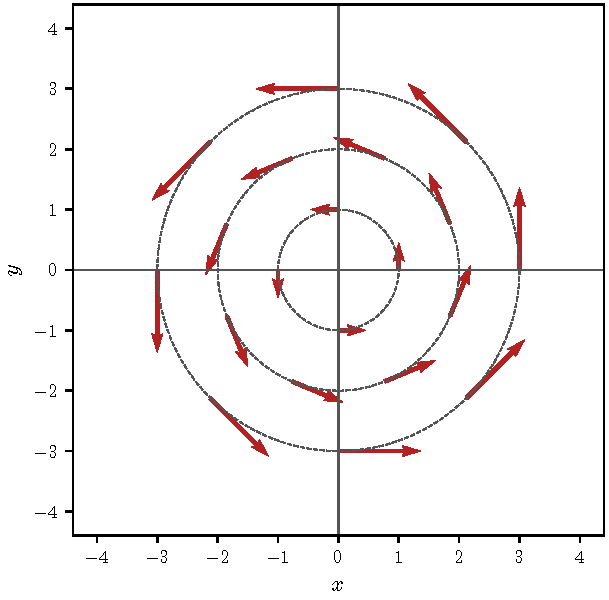
\includegraphics[width=0.48\linewidth]{rotation_field}
  \caption{$\vF(x,y)=\ip{-y,x}$ (arrows scaled by $\frac{1}{2.2}$). Each arrow is
  tangent to the dashed circle through its base point, with length equal to the
  radius.}
  \label{fig:rotation}
\end{figure}

\begin{exercise}[Slides, Exercise 1]\label{ex:exercise1}
Sketch the vector field $\vF(x,y)=y\,\vi+\frac12(y-x)\,\vj$ by drawing its vectors at
the nine points $(x,y)$ with $x,y\in\{-1,0,1\}$.
\end{exercise}
\begin{solution}
\step{1}{Compute.} $\vF(x,y)=\ip{y,\;\frac{y-x}{2}}$:
\begin{center}
\renewcommand{\arraystretch}{1.2}
\begin{tabular}{c|ccc}
\toprule
 & $x=-1$ & $x=0$ & $x=1$\\
\midrule
$y=1$ & $\ip{1,1}$ & $\ip{1,\frac12}$ & $\ip{1,0}$\\
$y=0$ & $\ip{0,\frac12}$ & $\ip{0,0}$ & $\ip{0,-\frac12}$\\
$y=-1$ & $\ip{-1,0}$ & $\ip{-1,-\frac12}$ & $\ip{-1,-1}$\\
\bottomrule
\end{tabular}
\end{center}
For instance at $(-1,1)$: $\ip{1,\frac{1-(-1)}{2}}=\ip{1,1}$; at $(1,0)$:
$\ip{0,\frac{0-1}{2}}=\ip{0,-\frac12}$.
\step{2}{Draw.} Attach each arrow to its point (Figure~\ref{fig:exercise1}).
The field vanishes at the origin; above the $x$-axis the arrows point right,
below they point left, and on the $x$-axis they are vertical. The overall
pattern is a clockwise swirl around the origin. (Compare with the GeoGebra
answer linked on the slide.)
\end{solution}

\begin{figure}[H]
  \centering
  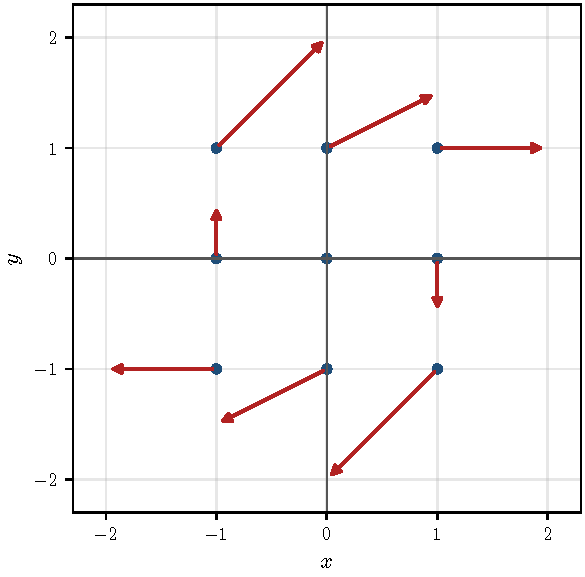
\includegraphics[width=0.46\linewidth]{exercise1}
  \caption{Exercise 1: $\vF=y\,\vi+\frac12(y-x)\,\vj$ at the nine indicated
  points (true length, no scaling).}
  \label{fig:exercise1}
\end{figure}

\begin{exercise}[Slides, Exercise 2]\label{ex:exercise2}
Match each vector field with its plot on the slide (four coloured panels):
\[
\text{A. }\vF=\ip{-\tfrac12,\tfrac12}\quad
\text{B. }\vF=\ip{\tfrac x2,\tfrac y2}\quad
\text{C. }\vF=\ip{1,\sin y}\quad
\text{D. }\vF=-\frac{\ip{x,y}}{\sqrt{x^2+y^2}} .
\]
\end{exercise}
\begin{solution}
Identify one distinguishing feature of each field first.
\begin{itemize}
\item \textbf{A} is \emph{constant}: every arrow is the same vector, pointing up and
      to the left at $135^\circ$. $\Rightarrow$ the \textbf{blue} panel (top right),
      where all arrows are identical and parallel.
\item \textbf{B} $=\frac12\vx$ is \emph{radial outward} with length $\frac12r$, so the
      arrows grow as we move away from the origin. $\Rightarrow$ the
      \textbf{orange} panel (bottom left).
\item \textbf{C} has $x$-component always $1$, so every arrow points to the right.
      Its $y$-component $\sin y$ is $0$ on the lines $y=0,\pm\pi$ (horizontal arrows),
      positive for $0<y<\pi$ and negative for $-\pi<y<0$; the arrows do not
      depend on $x$. $\Rightarrow$ the \textbf{yellow} panel (bottom right), whose
      rows of arrows are identical across each horizontal line.
\item \textbf{D} $=-\vx/\norm{\vx}$ has length $1$ everywhere and points
      \emph{toward the origin}. $\Rightarrow$ the \textbf{green} panel (top left),
      radial with arrows of equal length.
\end{itemize}
Answer: A--blue, B--orange, C--yellow, D--green
(Figure~\ref{fig:exercise2} redraws each field with its formula).
\end{solution}

\begin{figure}[H]
  \centering
  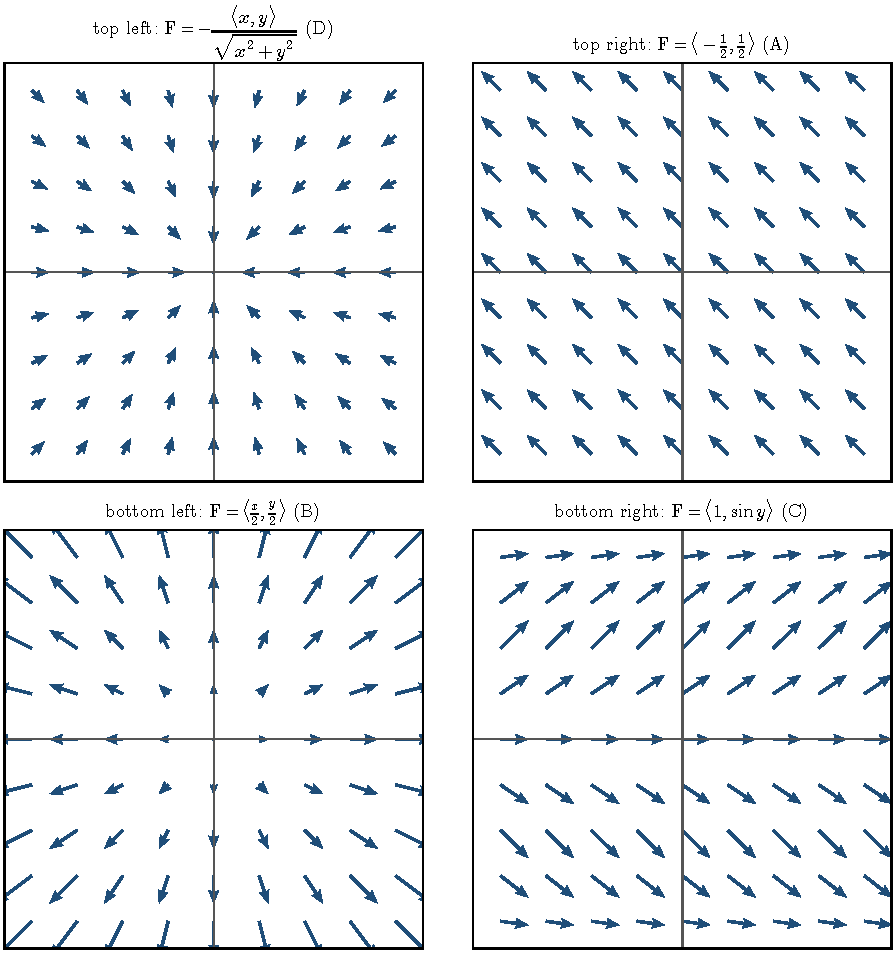
\includegraphics[width=0.78\linewidth]{exercise2}
  \caption{Exercise 2 redrawn: each panel is in the position of the
  corresponding coloured panel on the slide, labelled with its field.}
  \label{fig:exercise2}
\end{figure}

\begin{exercise}[Slides, Exercise 3]\label{ex:exercise3}
Which vector field has the plot shown on the slide (arrows in space, all
pointing upward and fanning outward away from the $z$-axis)?\\
A. $\vF=\ip{1,2,3}$\quad B. $\vF=\ip{1,2,z}$\quad C. $\vF=\ip{x,y,3}$\quad D. $\vF=\ip{x,y,z}$
\end{exercise}
\begin{solution}
\begin{itemize}
\item A is constant: all arrows would be parallel. The plot's arrows spread
      out, so not A.
\item B and D have $\vk$-component $z$, which is negative below the
      $xy$-plane, so some arrows would point \emph{down}; in the plot every arrow
      points up. Not B, not D. (D would be radial from the origin.)
\item C: the $\vk$-component is the constant $3>0$ (always up, same vertical
      size), while the horizontal part $\ip{x,y}$ points away from the $z$-axis
      and grows with the distance from it: exactly the fanning pattern.
\end{itemize}
Answer: \textbf{C}, $\vF(x,y,z)=\ip{x,y,3}$ (Figure~\ref{fig:exercise3}).
(On the slide, B--D are written as ``$\vF(x,y)$''; since they involve $z$ they
should read $\vF(x,y,z)$.)
\end{solution}

\begin{figure}[H]
  \centering
  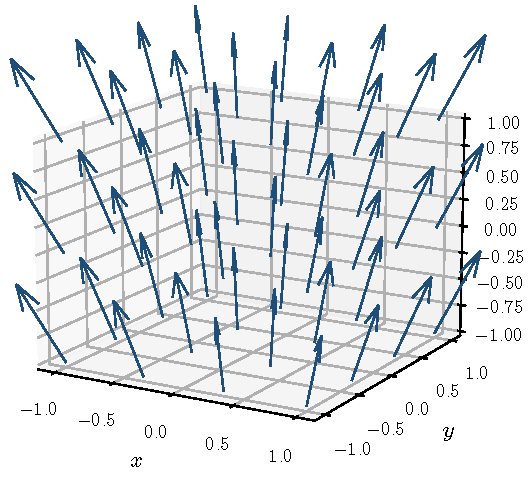
\includegraphics[width=0.5\linewidth]{exercise3}
  \caption{Exercise 3: $\vF(x,y,z)=\ip{x,y,3}$.}
  \label{fig:exercise3}
\end{figure}

\subsection{Computer-generated vector fields}

For anything but the simplest fields we let a computer draw the arrows,
usually scaled so they do not overlap. Figure~\ref{fig:computer} reproduces the
three examples on the slides. Notice how the formula is visible in the picture:
in $\ip{y,\sin x}$ the arrows are horizontal along the lines $x=k\pi$ (where
$\sin x=0$), and in $\ip{\ln(1+y^2),\ln(1+x^2)}$ both components are $\ge0$, so
every arrow points into the first-quadrant directions (right and/or up).

\begin{figure}[H]
  \centering
  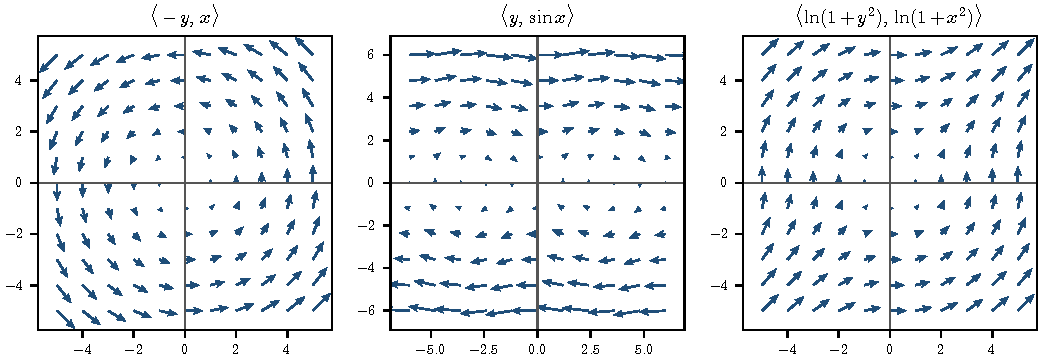
\includegraphics[width=\linewidth]{computer_fields}
  \caption{Slides, Figures 6--8: $\ip{-y,x}$, $\ip{y,\sin x}$ and
  $\ip{\ln(1+y^2),\ln(1+x^2)}$.}
  \label{fig:computer}
\end{figure}

\interactive{https://www.desmos.com/calculator/cho2h9ztfa}{Open the slide's Desmos graph}
(a gradient field drawn as arrows on a grid; see Example~\ref{ex:7.2}); edit
the two components to draw any other planar field. Appendix~\ref{app:interactive}
explains how to do the same in Python.

\subsection{Fields in physics}

\textbf{Velocity fields} (Slides, \emph{Application}). Wind patterns, ocean
currents and the airflow past an airfoil are described by assigning to each
point the velocity of the fluid there; the arrows on the slide's San Francisco
Bay and Nova Scotia maps are exactly such vectors.

\begin{example}[Gravitational field]\label{ex:gravity}
By Newton's law of gravitation, a mass $M$ at the origin attracts a mass $m$
at $\vx=\ip{x,y,z}$ with a force of magnitude $\dfrac{mMG}{\norm{\vx}^2}$ directed
toward the origin. Write the force as a vector field.
\end{example}
\begin{solution}
The unit vector from $\vx$ toward the origin is $-\vx/\norm{\vx}$. Multiplying by
the magnitude,
\[
  \vF(\vx)=-\frac{mMG}{\norm{\vx}^2}\cdot\frac{\vx}{\norm{\vx}}=-\frac{mMG}{\norm{\vx}^3}\,\vx
  =\ip{\frac{-mMGx}{(x^2+y^2+z^2)^{3/2}},\frac{-mMGy}{(x^2+y^2+z^2)^{3/2}},\frac{-mMGz}{(x^2+y^2+z^2)^{3/2}}}.
\]
All arrows point toward the origin and shrink like $1/r^2$
(Figure~\ref{fig:gravity}). The \emph{electric} force exerted by a charge $Q$ at
the origin on a charge $q$ at $\vx$, $\vF=\dfrac{\varepsilon qQ}{\norm{\vx}^3}\vx$
(Coulomb's law), has the same shape, pointing away from the origin when
$qQ>0$.
\end{solution}

\begin{figure}[H]
  \centering
  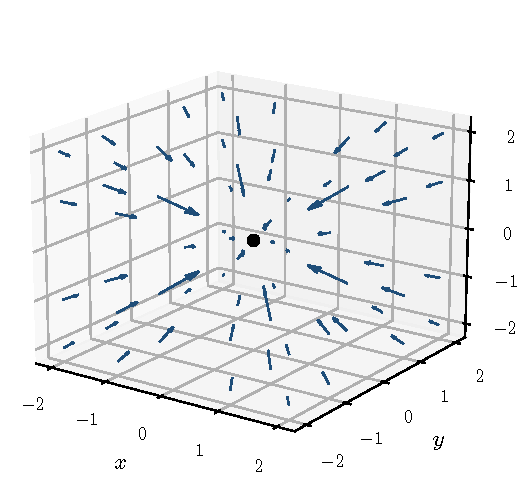
\includegraphics[width=0.48\linewidth]{gravity_field}
  \caption{An inverse-square field $\vF=-\vx/\norm{\vx}^3$: arrows point toward
  the origin and are much longer nearby.}
  \label{fig:gravity}
\end{figure}

\begin{example}\label{ex:zk}
Describe the vector field $\vF(x,y,z)=z\,\vk$.
\end{example}
\begin{solution}
Every arrow is vertical. At height $z$ its length is $|z|$: arrows point up
above the $xy$-plane, down below it, and vanish on the $xy$-plane. All points
at the same height carry the same arrow, since $\vF$ does not depend on $x$ or
$y$.
\end{solution}

% =====================================================================
\section{Gradient Fields}\label{ch:gradfields}
% =====================================================================

\begin{definition}[Gradient vector field; Slides, Definition 3]\label{def:gradfield}
If $f$ is a scalar function of two variables, its gradient
\[
  \grad f(x,y)=\ip{f_x(x,y),\,f_y(x,y)}
\]
is a vector field on $\R^2$, called a \emph{gradient vector field}. Likewise, if
$f$ is a scalar function of three variables, its gradient
$\grad f(x,y,z)=\ip{f_x,\,f_y,\,f_z}$ is a vector field on $\R^3$.
\end{definition}

So every differentiable scalar function produces a vector field. By Lecture
Notes No.~6, the arrows of a gradient field (i) point in the direction of
fastest increase of $f$, (ii) have length equal to that fastest rate, and
(iii) are perpendicular to the level curves of $f$.

\begin{example}[Slides, Example 7.2]\label{ex:7.2}
Find the gradient vector field of $f(x,y)=x^2y-y^3$.
\end{example}
\begin{solution}
$f_x=2xy$ (treat $y$ as constant) and $f_y=x^2-3y^2$ (treat $x$ as constant). Hence
\[
  \grad f(x,y)=\ip{2xy,\;x^2-3y^2}=2xy\,\vi+(x^2-3y^2)\,\vj .
\]
Figure~\ref{fig:gradfield} draws this field on top of the level curves of $f$
(see also the Desmos graph linked on the slide). Every arrow crosses the level
curves at a right angle and points toward larger values of $f$; arrows are long
where the level curves are crowded together. At the origin
$\grad f=\vzero$ (a saddle-like critical point; the level curve $f=0$ consists
of the three lines $y=0$ and $y=\pm x$).
\end{solution}

\begin{figure}[H]
  \centering
  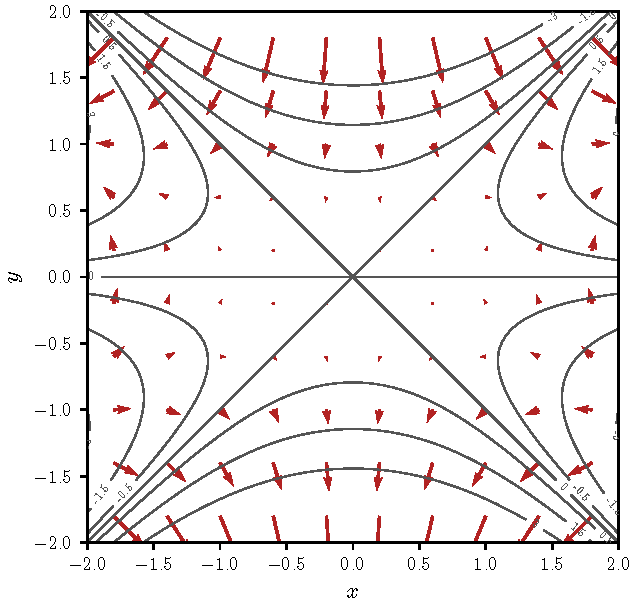
\includegraphics[width=0.55\linewidth]{gradient_field}
  \caption{Example 7.2: the gradient field $\grad f=\ip{2xy,x^2-3y^2}$ (red,
  scaled) over level curves of $f=x^2y-y^3$ (grey). Gradient vectors are
  perpendicular to the level curves.}
  \label{fig:gradfield}
\end{figure}

\begin{example}\label{ex:gradfield3}
Find the gradient field of (a) $f(x,y,z)=\frac12\ln(x^2+y^2+z^2)$ and
(b) $g(x,y,z)=\dfrac{c}{\sqrt{x^2+y^2+z^2}}$, $c$ a constant, and describe them.
\end{example}
\begin{solution}
Let $r=\norm{\vx}=\sqrt{x^2+y^2+z^2}$.

\textbf{(a)} By the chain rule,
$f_x=\frac12\cdot\frac{2x}{x^2+y^2+z^2}=\frac{x}{x^2+y^2+z^2}$, and similarly for $y,z$:
\[
  \grad f=\ip{\frac{x}{x^2+y^2+z^2},\,\frac{y}{x^2+y^2+z^2},\,\frac{z}{x^2+y^2+z^2}}=\frac{\vx}{r^2}.
\]
This is the field of Slides, Example~7.5: radial, pointing away from the
origin, with length $1/r$.

\textbf{(b)} Using $\grad(1/r)=-\vx/r^3$ (Lecture Notes No.~6, \S3.5, ``Gradient of
distance''), $\grad g=-c\,\vx/r^3$. With $c=mMG$ this is exactly the
gravitational field of Example~\ref{ex:gravity}. So gravity is a gradient field:
$\vF=\grad\!\left(\frac{mMG}{r}\right)$.
\end{solution}

\begin{example}\label{ex:gradfield-more}
Find the gradient fields of (a) $f=x^2+y^2$, (b) $f=e^x\cos y$,
(c) $f=xyz+z^2$.
\end{example}
\begin{solution}
\textbf{(a)} $\grad f=\ip{2x,2y}=2\vx$: radial outward, length $2r$.
\textbf{(b)} $\grad f=\ip{e^x\cos y,\,-e^x\sin y}$.
\textbf{(c)} $\grad f=\ip{yz,\;xz,\;xy+2z}$.
\end{solution}

\begin{remark}[The reverse question]
Computing $\grad f$ from $f$ is routine. The interesting question, and the
subject of the next chapter, is the \emph{reverse}: given a vector field $\vF$,
is it the gradient of some function, and if so, which one? For example, is
$\ip{yz,\,xz,\,xy+2z}$ a gradient? By (c) above, yes. Is $\ip{x^3y,\,xy}$? We
will see that it is not.
\end{remark}

% =====================================================================
\section{Conservative Vector Fields and Potential Functions}\label{ch:conservative}
% =====================================================================

\subsection{Definition}

Some vector fields can be represented as the gradients of differentiable
functions and some cannot. Those that can are called \emph{conservative}
(Slides).

\begin{definition}[Conservative field; Slides, Definition 4]\label{def:conservative}
A vector field $\vF$ is called \emph{conservative} when there exists a
differentiable function $f$ such that $\vF=\grad f$. The function $f$ is called a
\emph{potential function} for $\vF$.
\end{definition}

\begin{remark}
(1) If $f$ is a potential for $\vF$, so is $f+C$ for every constant $C$, since
$\grad C=\vzero$. On a connected domain these are \emph{all} the potentials, so
the answer to ``find the potential'' is always ``$f+C$''.
(2) The name comes from physics: for a conservative force, mechanical energy
is conserved. Physicists usually write $\vF=-\grad U$, with $U=-f$ the
\emph{potential energy}; e.g.\ gravity is $\grad(mMG/r)$ (Example~\ref{ex:gradfield3}).
\end{remark}

\begin{example}[Slides, Example 7.3]\label{ex:7.3}
The vector field $\vF(x,y)=\ip{3x^2,\,y}$ is conservative, since
$f(x,y)=x^3+\frac12y^2$ satisfies $\grad f=\ip{3x^2,\,y}=\vF$.
\end{example}
\begin{solution}
Verification: $f_x=3x^2$ and $f_y=\frac12\cdot2y=y$, so $\grad f=\vF$.\checkok
How was $f$ found? Each component depends on one variable only, so
$f=\int3x^2\,\dd x+\int y\,\dd y=x^3+\frac12y^2$ (plus a constant). The general
method is in Section~\ref{sec:potential}.
\end{solution}

\subsection{Why there is a test: mixed partials}

Suppose $\vF=\ip{M,N}=\grad f$, i.e.\ $M=f_x$ and $N=f_y$, where $f$ has
continuous second partial derivatives. Then by Clairaut's theorem
(Theorem~\ref{thm:clairaut})
\[
  M_y=(f_x)_y=f_{xy}=f_{yx}=(f_y)_x=N_x .
\]
So $M_y=N_x$ is a \emph{necessary} condition for $\ip{M,N}$ to be conservative.
On a disk (or any simply connected region) it is also \emph{sufficient}.

\begin{theorem}[Test for conservative vector field in the plane; Slides, Theorem 1]\label{thm:test2}
Let $M$ and $N$ have continuous first partial derivatives on an open disk $R$.
The vector field $\vF(x,y)=M\,\vi+N\,\vj$ is conservative on $R$ if and only if
\[
  \pd{N}{x}=\pd{M}{y}\qquad(\text{i.e. } N_x=M_y).
\]
\end{theorem}

\begin{example}[Slides, Example 7.4]\label{ex:7.4}
Determine whether the vector field is conservative:
(1) $\vF(x,y)=\ip{x^3y,\,xy}$;\quad (2) $\vF(x,y)=\ip{2x,\,y}$.
\end{example}
\begin{solution}
\textbf{(1)} $M=x^3y$, $N=xy$: $M_y=x^3$ and $N_x=y$. These are not equal (e.g.\ at
$(1,0)$: $1\neq0$), so $\vF$ is \textbf{not} conservative.

\textbf{(2)} $M=2x$, $N=y$: $M_y=0=N_x$. The partials are continuous on all of
$\R^2$, so $\vF$ \textbf{is} conservative. (Indeed $f=x^2+\frac12y^2$.)
\end{solution}

\begin{warning}
$M_y=N_x$ must hold as an \emph{identity}, for all $(x,y)$ in the region, not
just at one point. In (1), $x^3=y$ holds along a curve, but that does not
make $\vF$ conservative.
\end{warning}

\begin{theorem}[Test for conservative vector field in space; Slides, Theorem 2]\label{thm:test3}
Let $M$, $N$ and $P$ have continuous first partial derivatives on an open
sphere (ball) $Q$. The vector field $\vF(x,y,z)=M\,\vi+N\,\vj+P\,\vk$ is
conservative on $Q$ if and only if
\[
  M_y=N_x,\qquad N_z=P_y,\qquad P_x=M_z .
\]
\end{theorem}

\begin{remark}[Remembering the three conditions]
Each condition pairs two components and two variables: the
$(x,y)$-pair $M_y=N_x$, the $(y,z)$-pair $N_z=P_y$, the $(z,x)$-pair $P_x=M_z$.
They come from $f_{xy}=f_{yx}$, $f_{yz}=f_{zy}$, $f_{zx}=f_{xz}$. (They say that
the \emph{curl} of $\vF$, $\ip{P_y-N_z,\,M_z-P_x,\,N_x-M_y}$, is zero.)
\end{remark}

\begin{example}[Slides, Example 7.5]\label{ex:7.5}
Determine whether the vector field is conservative:
\[
  \vF(x,y,z)=\frac{x}{x^2+y^2+z^2}\,\vi+\frac{y}{x^2+y^2+z^2}\,\vj+\frac{z}{x^2+y^2+z^2}\,\vk .
\]
\end{example}
\begin{solution}
Write $\rho=x^2+y^2+z^2$, so $M=x/\rho$, $N=y/\rho$, $P=z/\rho$. Quotient rule,
remembering that the numerator of $M$ does not involve $y$ or $z$, etc.:

\step{1}{$M_y$ and $N_x$.}
\[
  M_y=\frac{\rho\cdot0-x\cdot2y}{\rho^2}=\frac{-2xy}{\rho^2},\qquad
  N_x=\frac{\rho\cdot0-y\cdot2x}{\rho^2}=\frac{-2xy}{\rho^2}.\qquad\text{So }M_y=N_x.
\]
\step{2}{$N_z$ and $P_y$.}
\[
  N_z=\frac{\rho\cdot0-y\cdot2z}{\rho^2}=\frac{-2yz}{\rho^2},\qquad
  P_y=\frac{\rho\cdot0-z\cdot2y}{\rho^2}=\frac{-2yz}{\rho^2}.\qquad\text{So }N_z=P_y.
\]
\step{3}{$P_x$ and $M_z$.}
\[
  P_x=\frac{-2xz}{\rho^2},\qquad M_z=\frac{-2xz}{\rho^2}.\qquad\text{So }P_x=M_z.
\]
By Theorem~\ref{thm:test3}, $\vF$ is conservative, i.e. a potential function
$f$ with $\grad f=\vF$ exists. (By Example~\ref{ex:gradfield3}(a),
$f=\frac12\ln(x^2+y^2+z^2)+C$; the slides derive it in Example~7.6 below.)
\end{solution}

\begin{remark}[About the domain]
$\vF$ is undefined at the origin, so strictly its domain is
$\R^3\setminus\{\vzero\}$, not an open ball. The conclusion is still correct:
the test works on any \emph{simply connected} region, and $\R^3$ minus a point is
simply connected (every loop can be shrunk to a point while avoiding the
origin). On every ball not containing the origin, Theorem~\ref{thm:test3}
applies directly.
\end{remark}

\subsection{Finding a potential function}\label{sec:potential}

If $\vF=\ip{M,N,P}$ is conservative, there is $f$ with
$\ip{f_x,f_y,f_z}=\ip{M,N,P}$, i.e.
\[
  f_x=M,\qquad f_y=N,\qquad f_z=P .
\]
We find $f$ by \emph{reversing partial differentiation}: integrate one equation
and use the other two to determine the missing function (Slides).

\begin{strategy}{Strategy (finding the potential function; Slides).}
\begin{enumerate}
\item \textbf{Integrate with respect to $x$.} From $f_x=M$:
      \[ f(x,y,z)=\int M\,\dd x+g(y,z), \]
      where $g(y,z)$ is (at this point) an unknown function.
\item \textbf{Differentiate with respect to $y$.} Differentiate the $f$ from
      Step~1 with respect to $y$ and set $f_y=N$. Solve for $g_y(y,z)$, then
      integrate with respect to $y$. This determines $g(y,z)$ up to an unknown
      function $h(z)$.
\item \textbf{Differentiate with respect to $z$.} Substitute $g$ into $f$,
      differentiate with respect to $z$ and set $f_z=P$. Solve for $h'(z)$,
      then integrate to obtain $h(z)$.
\item \textbf{Assemble and check} $\grad f=\vF$. Answer: $f+C$.
\end{enumerate}
In two variables stop after Step~2, with $g=g(y)$ a function of $y$ only, whose
derivative $g'(y)$ is found from $f_y=N$.
\end{strategy}

\begin{remark}[A built-in alarm]
In Step~2, $g_y$ must turn out to depend on $y$ and $z$ only (and in Step~3,
$h'$ on $z$ only). If an $x$ survives, either you made an algebra error or $\vF$
is not conservative (Example~\ref{ex:not-cons}).
\end{remark}

\begin{example}[Two variables]\label{ex:pot2d}
Show that $\vF(x,y)=\ip{3+2xy,\;x^2-3y^2}$ is conservative and find a potential
function.
\end{example}
\begin{solution}
\step{1}{Test.} $M_y=2x$ and $N_x=2x$; the partials are continuous on $\R^2$,
so $\vF$ is conservative.
\step{2}{Integrate $f_x=M$ in $x$.} $f=\int(3+2xy)\,\dd x=3x+x^2y+g(y)$.
\step{3}{Use $f_y=N$.} $f_y=x^2+g'(y)$ must equal $x^2-3y^2$, so $g'(y)=-3y^2$ (no
$x$: good) and $g(y)=-y^3+K$.
\step{4}{Answer.} $f(x,y)=3x+x^2y-y^3+K$.
\step{5}{Check.} $f_x=3+2xy$\checkok, $f_y=x^2-3y^2$\checkok.
\end{solution}

\begin{example}[Slides, Example 7.6]\label{ex:7.6}
Find the potential function for
$\vF(x,y,z)=\dfrac{x}{x^2+y^2+z^2}\,\vi+\dfrac{y}{x^2+y^2+z^2}\,\vj+\dfrac{z}{x^2+y^2+z^2}\,\vk$.
\end{example}
\begin{solution}
$\vF$ is conservative by Example~\ref{ex:7.5}.

\step{1}{Integrate with respect to $x$.} $f_x=M=\dfrac{x}{x^2+y^2+z^2}$. Substituting
$w=x^2+y^2+z^2$, $\dd w=2x\,\dd x$ ($y,z$ fixed):
\[
  f(x,y,z)=\int\frac{x}{x^2+y^2+z^2}\,\dd x=\frac12\ln\abs{x^2+y^2+z^2}+g(y,z).
\]
\step{2}{Differentiate with respect to $y$.}
\[
  f_y=\frac12\cdot\frac{2y}{x^2+y^2+z^2}+g_y(y,z)=\frac{y}{x^2+y^2+z^2}+g_y(y,z).
\]
Comparing with $f_y=N=\dfrac{y}{x^2+y^2+z^2}$ gives $g_y(y,z)=0$. Integrating with
respect to $y$: $g(y,z)=\int0\,\dd y=C_1+h(z)$ for some constant $C_1$ and some
function $h(z)$. Hence
\[
  f(x,y,z)=\frac12\ln\abs{x^2+y^2+z^2}+C_1+h(z).
\]
\step{3}{Differentiate with respect to $z$.}
$f_z=\dfrac{z}{x^2+y^2+z^2}+h'(z)$. Comparing with $f_z=P=\dfrac{z}{x^2+y^2+z^2}$ gives
$h'(z)=0$, so $h(z)=\int0\,\dd z=C_2$. Hence
\[
  f(x,y,z)=\tfrac12\ln\abs{x^2+y^2+z^2}+C_1+C_2 .
\]
\textbf{Answer.} The potential function is of the form
\[
  f(x,y,z)=\frac12\ln\left(x^2+y^2+z^2\right)+C,
\]
$C$ an arbitrary constant. (The absolute value can be dropped since
$x^2+y^2+z^2>0$ on the domain.)
\end{solution}

\begin{exercise}[Slides, Exercise 4]\label{ex:exercise4}
Determine whether $\vF(x,y,z)=y^2\,\vi+(2xy+e^{3z})\,\vj+3ye^{3z}\,\vk$ is
conservative. If it is, find a potential function for $\vF$.
\end{exercise}
\begin{solution}
$M=y^2$, $N=2xy+e^{3z}$, $P=3ye^{3z}$.

\step{1}{Test (Theorem~\ref{thm:test3}).}
\[
  M_y=2y=N_x,\qquad N_z=3e^{3z}=P_y,\qquad P_x=0=M_z .
\]
All partials are continuous on $\R^3$, so $\vF$ \textbf{is conservative}.

\step{2}{Integrate $f_x=y^2$ in $x$.} $f=xy^2+g(y,z)$.

\step{3}{Differentiate in $y$.} $f_y=2xy+g_y(y,z)$. Setting equal to
$N=2xy+e^{3z}$: $g_y(y,z)=e^{3z}$. Integrate in $y$ ($z$ fixed):
$g(y,z)=ye^{3z}+h(z)$. So $f=xy^2+ye^{3z}+h(z)$.

\step{4}{Differentiate in $z$.} $f_z=3ye^{3z}+h'(z)$. Setting equal to
$P=3ye^{3z}$: $h'(z)=0$, $h(z)=C$.

\textbf{Answer.} $f(x,y,z)=xy^2+ye^{3z}+C$.

\step{5}{Check.} $\grad f=\ip{y^2,\;2xy+e^{3z},\;3ye^{3z}}=\vF$.\checkok
\end{solution}

\begin{example}\label{ex:pot3d}
Find a potential for $\vF=\ip{2xy+z^2,\;x^2,\;2xz+\cos z}$.
\end{example}
\begin{solution}
\step{1}{Test.} $M_y=2x=N_x$; $N_z=0=P_y$; $P_x=2z=M_z$. Conservative on $\R^3$.
\step{2}{$x$-integration.} $f=x^2y+xz^2+g(y,z)$.
\step{3}{$y$.} $f_y=x^2+g_y=x^2\Rightarrow g_y=0\Rightarrow g=h(z)$.
\step{4}{$z$.} $f_z=2xz+h'(z)=2xz+\cos z\Rightarrow h'(z)=\cos z\Rightarrow h=\sin z+C$.

\textbf{Answer.} $f=x^2y+xz^2+\sin z+C$. Check: $\grad f=\ip{2xy+z^2,\,x^2,\,2xz+\cos z}$.\checkok
\end{solution}

\begin{example}[What goes wrong if $\vF$ is not conservative]\label{ex:not-cons}
Try to find a potential for $\vF=\ip{x^3y,\;xy}$ (Example~\ref{ex:7.4}(1)).
\end{example}
\begin{solution}
Step~1 gives $f=\frac14x^4y+g(y)$. Step~2: $f_y=\frac14x^4+g'(y)$ should equal $xy$, so
$g'(y)=xy-\frac14x^4$. But $g'(y)$ is supposed to depend on $y$ only, and the
right-hand side depends on $x$. Contradiction: no potential exists, in
agreement with the test $M_y=x^3\neq y=N_x$.
\end{solution}

\begin{remark}[A quick alternative for checking]
Integrate each component in its own variable and merge the terms:
$\int M\,\dd x$, $\int N\,\dd y$, $\int P\,\dd z$, keeping every distinct term
once. For Exercise~4: $\int y^2\,\dd x=xy^2$, $\int(2xy+e^{3z})\,\dd y=xy^2+ye^{3z}$,
$\int3ye^{3z}\,\dd z=ye^{3z}$; merging gives $xy^2+ye^{3z}$. This is fast but
\emph{must} be followed by the check $\grad f=\vF$, because it can silently
produce a wrong answer when $\vF$ is not conservative. On an exam, show the
three-step method.
\end{remark}

\subsection{A caveat: the shape of the domain}\label{sec:caveat}

Theorems~\ref{thm:test2} and~\ref{thm:test3} are stated on a disk or a ball.
They remain true on any simply connected region, but can fail on regions with
holes.

\begin{example}[The vortex field]\label{ex:vortex}
Let $\vF(x,y)=\dfrac{-y}{x^2+y^2}\,\vi+\dfrac{x}{x^2+y^2}\,\vj$ on the punctured
plane $\R^2\setminus\{(0,0)\}$. Show that $M_y=N_x$ everywhere on this domain.
\end{example}
\begin{solution}
\[
  M_y=\frac{(x^2+y^2)(-1)-(-y)(2y)}{(x^2+y^2)^2}=\frac{y^2-x^2}{(x^2+y^2)^2},\qquad
  N_x=\frac{(x^2+y^2)(1)-x(2x)}{(x^2+y^2)^2}=\frac{y^2-x^2}{(x^2+y^2)^2}.
\]
They agree. Nevertheless, $\vF$ is \emph{not} conservative on the punctured
plane. Suppose, for contradiction, that $\vF=\grad f$ there. Walk once around
the unit circle, $\vr(t)=\ip{\cos t,\sin t}$, and let $g(t)=f(\cos t,\sin t)$.
By the chain rule (Lecture Notes No.~6, Theorem~1.11),
\[
  g'(t)=\grad f(\vr(t))\cdot\vr\,'(t)=\vF(\cos t,\sin t)\cdot\ip{-\sin t,\cos t}
  =\ip{-\sin t,\cos t}\cdot\ip{-\sin t,\cos t}=1 ,
\]
using $x^2+y^2=1$ on the circle. Hence $g(2\pi)-g(0)=\int_0^{2\pi}1\,\dd t=2\pi$.
But $\vr(2\pi)=\vr(0)$ is the same point, so $g(2\pi)=g(0)$: a contradiction.
The hole at the origin is responsible (Figure~\ref{fig:vortex}).

On the right half-plane $x>0$ (simply connected), $\vF=\grad\theta$ with
$\theta=\arctan(y/x)$ the polar angle (Lecture Notes No.~6,
Problem~5.11). Going once around the origin, the angle increases by $2\pi$ and
cannot return to its starting value; that is why no single potential exists
on the whole punctured plane.
\end{solution}

\begin{figure}[H]
  \centering
  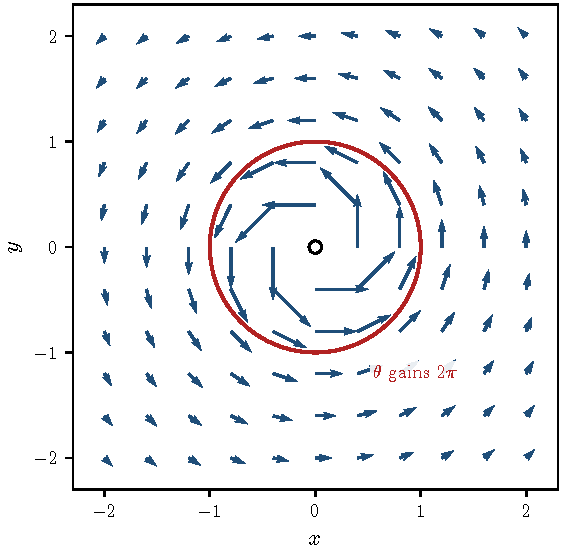
\includegraphics[width=0.46\linewidth]{vortex}
  \caption{The vortex field (arrow lengths capped near the origin). $M_y=N_x$
  everywhere, yet a would-be potential would have to increase by $2\pi$ on each
trip around the red circle, which is impossible.}
  \label{fig:vortex}
\end{figure}

\begin{keybox}{Summary: deciding and finding}
\begin{enumerate}
\item Compute the cross partials ($M_y,N_x$ in 2D; all three pairs in 3D).
\item If any pair differs: \textbf{not conservative}. Stop.
\item If all pairs agree and the domain is a disk/ball/all of $\R^n$ (or simply
      connected): \textbf{conservative}. Find $f$ by the three-step method and
      check $\grad f=\vF$.
\end{enumerate}
\end{keybox}

% =====================================================================
\section{Practice Problems with Complete Solutions}\label{ch:practice}
% =====================================================================

The problems follow the patterns of the slides: sketching and matching vector
fields (Example~7.1, Exercises~1--3), computing gradient fields
(Example~7.2), the component test in the plane and in space
(Examples~7.4--7.5) and the three-step potential method (Example~7.6,
Exercise~4). Problems marked $(*)$ go further. Try each problem before reading
its solution.

% ---------------------------------------------------------------------
\subsection{Sketching, describing and matching vector fields}

\begin{problem}\label{q:sketch}
Sketch $\vF(x,y)=\frac12x\,\vi+\frac12y\,\vj$ at the points $(\pm1,0)$, $(0,\pm1)$,
$(\pm1,\pm1)$ and $(\pm2,0)$, and describe the field.
\end{problem}
\begin{solution}
$\vF(x,y)=\frac12\ip{x,y}=\frac12\vx$:
\begin{center}
\renewcommand{\arraystretch}{1.2}
\begin{tabular}{cccccc}
\toprule
$(x,y)$ & $(1,0)$ & $(0,1)$ & $(1,1)$ & $(-1,1)$ & $(2,0)$\\
$\vF$ & $\ip{\frac12,0}$ & $\ip{0,\frac12}$ & $\ip{\frac12,\frac12}$ & $\ip{-\frac12,\frac12}$ & $\ip{1,0}$\\
\bottomrule
\end{tabular}
\end{center}
(and symmetrically at the other points, e.g. $\vF(-1,0)=\ip{-\frac12,0}$,
$\vF(-1,-1)=\ip{-\frac12,-\frac12}$). Every arrow points directly away from the
origin (it is a positive multiple of the position vector) and has length
$\frac12r$: a \emph{radial outward} field growing linearly with distance, like the
orange panel of Exercise~2.
\end{solution}

\begin{problem}\label{q:saddle}
Describe the field $\vF(x,y)=\ip{x,-y}$. Where is it horizontal? vertical? zero?
\end{problem}
\begin{solution}
$\vF=\vzero$ only at the origin. On the $x$-axis ($y=0$), $\vF=\ip{x,0}$ is
horizontal and points \emph{away} from the origin; on the $y$-axis ($x=0$),
$\vF=\ip{0,-y}$ is vertical and points \emph{toward} the origin. In the first
quadrant arrows point right and down, etc. Length $\norm{\vF}=\sqrt{x^2+y^2}=r$.
The picture is a ``saddle'' flow: in along the $y$-axis, out along the
$x$-axis, following the hyperbolas $xy=\text{const}$. (It is
$\grad\left(\frac12x^2-\frac12y^2\right)$.)
\end{solution}

\begin{problem}\label{q:match}
Match the fields with the plots I--IV of Figure~\ref{fig:matchpractice}.\\
A. $\vF=\ip{y,-x}$\qquad B. $\vF=\ip{2,1}$\qquad C. $\vF=\ip{x,-y}$\qquad D. $\vF=\ip{y,0}$
\end{problem}

\begin{figure}[H]
  \centering
  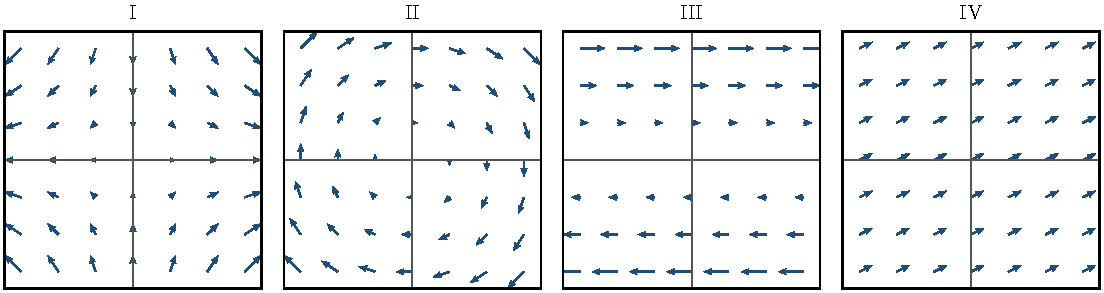
\includegraphics[width=\linewidth]{matching_practice}
  \caption{Plots for Problem~\ref{q:match}.}
  \label{fig:matchpractice}
\end{figure}

\begin{solution}
\begin{itemize}
\item B is constant: all arrows identical. Only plot \textbf{IV}.
\item D $=\ip{y,0}$ is always horizontal, pointing right above the $x$-axis and
      left below it, zero on it, longer farther from it. Plot \textbf{III}.
\item A $=\ip{y,-x}$ satisfies $\vF\cdot\vx=xy-yx=0$: tangent to circles. At
      $(0,1)$ it is $\ip{1,0}$ (to the right), so the rotation is
      \emph{clockwise}. Plot \textbf{II}.
\item C $=\ip{x,-y}$ is the saddle flow of Problem~\ref{q:saddle}. Plot \textbf{I}.
\end{itemize}
Answer: A--II, B--IV, C--I, D--III.
\end{solution}

\begin{problem}\label{q:3d}
Describe the vector field $\vF(x,y,z)=\ip{x,y,0}$ in space.
\end{problem}
\begin{solution}
Every arrow is horizontal (no $\vk$-component). At $(x,y,z)$ the arrow $\ip{x,y,0}$
points directly away from the $z$-axis, with length $\sqrt{x^2+y^2}$, the
distance to the $z$-axis. The field is the same in every horizontal plane: in
each plane $z=c$ it looks like the radial field $\ip{x,y}$. (Compare Exercise~3,
where the extra constant upward component $3\vk$ tilts every arrow upward.)
\end{solution}

% ---------------------------------------------------------------------
\subsection{Gradient fields}

\begin{problem}\label{q:grad1}
Find the gradient vector field of (a) $f(x,y)=xe^{xy}$;
(b) $f(x,y,z)=x\cos\left(\dfrac yz\right)$.
\end{problem}
\begin{solution}
\textbf{(a)} Product and chain rule: $f_x=e^{xy}+x\cdot ye^{xy}=(1+xy)e^{xy}$,
$f_y=x\cdot xe^{xy}=x^2e^{xy}$. So $\grad f=\ip{(1+xy)e^{xy},\;x^2e^{xy}}$.

\textbf{(b)} $f_x=\cos\frac yz$;
$f_y=x\cdot\left(-\sin\frac yz\right)\cdot\frac1z=-\frac xz\sin\frac yz$;
$f_z=x\cdot\left(-\sin\frac yz\right)\cdot\left(-\frac{y}{z^2}\right)=\frac{xy}{z^2}\sin\frac yz$. Hence
\[
  \grad f=\ip{\cos\frac yz,\;-\frac xz\sin\frac yz,\;\frac{xy}{z^2}\sin\frac yz}.
\]
\end{solution}

\begin{problem}\label{q:grad2}
Let $f(x,y)=x^2-y^2$. Find $\grad f$, show that it is perpendicular to the level
curve $f=3$ at $(2,1)$, and identify the field among those of
Problem~\ref{q:match}.
\end{problem}
\begin{solution}
$\grad f=\ip{2x,-2y}$, so $\grad f(2,1)=\ip{4,-2}$. The level curve $x^2-y^2=3$ passes
through $(2,1)$; implicit differentiation gives $2x-2yy'=0$, $y'=x/y=2$, so a
tangent vector is $\ip{1,2}$, and $\ip{4,-2}\cdot\ip{1,2}=4-4=0$.\checkok\
$\grad f=2\ip{x,-y}$ is twice field C (plot~I): the saddle flow.
\end{solution}

% ---------------------------------------------------------------------
\subsection{Testing for conservative fields}

\begin{problem}\label{q:which}
Which of the following are conservative?\\
(a) $\ip{y,x}$\quad (b) $\ip{y,-x}$\quad (c) $\ip{2x,2y,2z}$\quad (d) $\ip{z,0,-x}$\quad
(e) $\ip{e^x\cos y,\,e^x\sin y}$\quad (f) $\ip{e^x\cos y,\,-e^x\sin y}$
\end{problem}
\begin{solution}
\begin{enumerate}[label=(\alph*)]
\item $M_y=1=N_x$: conservative ($f=xy$).
\item $M_y=1$, $N_x=-1$: \textbf{not} conservative.
\item All cross partials are $0$: conservative ($f=x^2+y^2+z^2$).
\item $P_x=-1$ but $M_z=1$: \textbf{not} conservative.
\item $M_y=-e^x\sin y$, $N_x=e^x\sin y$: these differ wherever $\sin y\neq0$, so
      \textbf{not} conservative.
\item $M_y=-e^x\sin y=N_x$: conservative ($f=e^x\cos y$).
\end{enumerate}
\end{solution}

\begin{problem}\label{q:notcons3}
Show that $\vF=\ip{xyz^2,\;x^2yz^2,\;x^2y^2z}$ is not conservative.
\end{problem}
\begin{solution}
$M_y=xz^2$ while $N_x=2xyz^2$. These are not identically equal (at $(1,0,1)$:
$1\neq0$). One failed condition is enough: $\vF$ is not conservative. (The
other conditions need not be checked; in fact $N_z=2x^2yz=P_y$ holds, which
shows that \emph{all three} must be verified before concluding ``conservative''.)
\end{solution}

\begin{problem}\label{q:const}
(a) Find the value of $a$ for which $\vF=\ip{3x^2y+ay,\;x^3+2x}$ is conservative.
(b) Find $a,b$ such that $\mathbf{G}=\ip{yz,\;axz,\;bxy+2z}$ is conservative.
\end{problem}
\begin{solution}
\textbf{(a)} $M_y=3x^2+a$ and $N_x=3x^2+2$, equal for all $(x,y)$ iff $a=2$. Then
$\vF=\grad(x^3y+2xy)$.

\textbf{(b)} $M_y=z$, $N_x=az\Rightarrow a=1$. $N_z=ax$, $P_y=bx\Rightarrow b=a=1$.
$P_x=by$, $M_z=y\Rightarrow b=1$. All consistent: $a=b=1$, and then $\mathbf{G}=\grad(xyz+z^2)$
(Problem~\ref{q:pot3a}).
\end{solution}

\begin{problem}[$*$]\label{q:radial2d}
Let $\vF=\dfrac{\ip{x,y}}{x^2+y^2}$ on the punctured plane. Show that $M_y=N_x$ and
that, unlike the vortex field of Example~\ref{ex:vortex}, this field \emph{is}
conservative on the whole punctured plane.
\end{problem}
\begin{solution}
$M_y=\dfrac{-2xy}{(x^2+y^2)^2}=N_x$. A potential defined on the entire punctured
plane is $f=\frac12\ln(x^2+y^2)$: $f_x=\frac{x}{x^2+y^2}$, $f_y=\frac{y}{x^2+y^2}$.\checkok\
So on a non-simply-connected region the component test is inconclusive: it
holds for both fields, but one is conservative and the other is not. To prove
conservativeness there, exhibit a potential.
\end{solution}

% ---------------------------------------------------------------------
\subsection{Finding potential functions}

\begin{problem}\label{q:pot2a}
Show that $\vF=\ip{2x-3y,\;-3x+4y-8}$ is conservative and find a potential.
\end{problem}
\begin{solution}
\step{1}{Test.} $M_y=-3=N_x$ (polynomials, continuous on $\R^2$): conservative.
\step{2}{Integrate in $x$.} $f=x^2-3xy+g(y)$.
\step{3}{Match $f_y$.} $f_y=-3x+g'(y)=-3x+4y-8\Rightarrow g'(y)=4y-8\Rightarrow g=2y^2-8y+K$.

\textbf{Answer.} $f=x^2-3xy+2y^2-8y+K$. Check: $f_x=2x-3y$\checkok, $f_y=-3x+4y-8$\checkok.
\end{solution}

\begin{problem}\label{q:pot2b}
Find a potential for $\vF=\ip{(1+xy)e^{xy},\;x^2e^{xy}}$.
\end{problem}
\begin{solution}
\step{1}{Test.} $M_y=xe^{xy}+(1+xy)xe^{xy}=(2x+x^2y)e^{xy}$;
$N_x=2xe^{xy}+x^2ye^{xy}=(2x+x^2y)e^{xy}$. Equal: conservative.
\step{2}{Integrate the \emph{easier} component.} Integrating $N$ in $y$ is easier
than $M$ in $x$: $f=\int x^2e^{xy}\,\dd y=xe^{xy}+g(x)$.
\step{3}{Match $f_x$.} $f_x=e^{xy}+xye^{xy}+g'(x)=(1+xy)e^{xy}\Rightarrow g'(x)=0$.

\textbf{Answer.} $f=xe^{xy}+K$ (compare Problem~\ref{q:grad1}(a)).
\emph{Tip:} the order of the three steps may be changed; start with whichever
component is easiest to integrate.
\end{solution}

\begin{problem}\label{q:pot2c}
Find a potential for $\vF=\ip{ye^x+\sin y,\;e^x+x\cos y}$.
\end{problem}
\begin{solution}
Test: $M_y=e^x+\cos y=N_x$. Integrate in $x$: $f=ye^x+x\sin y+g(y)$. Then
$f_y=e^x+x\cos y+g'(y)=N\Rightarrow g'(y)=0$. Answer: $f=ye^x+x\sin y+K$.
\end{solution}

\begin{problem}\label{q:pot2d}
Find a potential for $\vF=\ip{\ln y+2xy^3,\;3x^2y^2+\dfrac xy}$, $y>0$.
\end{problem}
\begin{solution}
Test: $M_y=\frac1y+6xy^2$, $N_x=6xy^2+\frac1y$: equal, and the half-plane $y>0$ is
simply connected. Integrate in $x$: $f=x\ln y+x^2y^3+g(y)$. Then
$f_y=\frac xy+3x^2y^2+g'(y)=N\Rightarrow g'(y)=0$. Answer: $f=x\ln y+x^2y^3+K$.
\end{solution}

\begin{problem}\label{q:pot3a}
Show that $\vF=\ip{yz,\;xz,\;xy+2z}$ is conservative and find a potential.
\end{problem}
\begin{solution}
\step{1}{Test.} $M_y=z=N_x$; $N_z=x=P_y$; $P_x=y=M_z$. Conservative on $\R^3$.
\step{2}{$x$.} $f=xyz+g(y,z)$.
\step{3}{$y$.} $f_y=xz+g_y=xz\Rightarrow g_y=0\Rightarrow g=h(z)$.
\step{4}{$z$.} $f_z=xy+h'(z)=xy+2z\Rightarrow h'(z)=2z\Rightarrow h=z^2+K$.

\textbf{Answer.} $f=xyz+z^2+K$.
\end{solution}

\begin{problem}\label{q:pot3b}
Find a potential for $\vF=\ip{1,\;\sin z,\;y\cos z}$.
\end{problem}
\begin{solution}
Test: $M_y=0=N_x$; $N_z=\cos z=P_y$; $P_x=0=M_z$. Conservative.\\
$x$: $f=x+g(y,z)$. $y$: $g_y=\sin z\Rightarrow g=y\sin z+h(z)$.
$z$: $f_z=y\cos z+h'(z)=y\cos z\Rightarrow h=K$.\\
\textbf{Answer.} $f=x+y\sin z+K$.
\end{solution}

\begin{problem}\label{q:pot3c}
Find a potential for $\vF=\ip{e^{yz},\;xze^{yz},\;xye^{yz}}$.
\end{problem}
\begin{solution}
Test: $M_y=ze^{yz}=N_x$; $N_z=xe^{yz}+xyze^{yz}=P_y$; $P_x=ye^{yz}=M_z$. Conservative.\\
$x$: $f=xe^{yz}+g(y,z)$. $y$: $f_y=xze^{yz}+g_y=xze^{yz}\Rightarrow g=h(z)$.
$z$: $f_z=xye^{yz}+h'(z)=xye^{yz}\Rightarrow h=K$.\\
\textbf{Answer.} $f=xe^{yz}+K$.
\end{solution}

\begin{problem}\label{q:hx}
Find all functions $h(x)$ for which $\vF=\ip{h(x)\,y,\;x^3+y}$ is conservative,
and find the corresponding potentials.
\end{problem}
\begin{solution}
$M_y=h(x)$ and $N_x=3x^2$, so we need $h(x)=3x^2$. Then
$f=\int3x^2y\,\dd x=x^3y+g(y)$, $f_y=x^3+g'(y)=x^3+y\Rightarrow g=\frac12y^2+K$.
Answer: $h(x)=3x^2$ and $f=x^3y+\frac12y^2+K$.
\end{solution}

% ---------------------------------------------------------------------
\subsection{Mixed exam-style problems}

\begin{problem}[$*$]\label{q:mixed1}
Let $\vF(x,y,z)=\ip{2x\cos y-2z^3,\;3+2ye^z-x^2\sin y,\;y^2e^z-6xz^2}$.
\begin{enumerate}[label=(\alph*)]
\item Show that $\vF$ is conservative.
\item Find the potential $f$ with $f(0,0,0)=1$.
\item In which direction does $f$ increase fastest at the origin, and how fast?
\end{enumerate}
\end{problem}
\begin{solution}
\textbf{(a)}
$M_y=-2x\sin y=N_x$;\quad $N_z=2ye^z=P_y$;\quad $P_x=-6z^2=M_z$. All continuous on
$\R^3$: conservative.

\textbf{(b)} \step{1}{$x$.} $f=\int(2x\cos y-2z^3)\,\dd x=x^2\cos y-2xz^3+g(y,z)$.
\step{2}{$y$.} $f_y=-x^2\sin y+g_y=3+2ye^z-x^2\sin y\Rightarrow g_y=3+2ye^z\Rightarrow
g=3y+y^2e^z+h(z)$.
\step{3}{$z$.} $f_z=-6xz^2+y^2e^z+h'(z)=y^2e^z-6xz^2\Rightarrow h'=0\Rightarrow h=K$.\\
So $f=x^2\cos y+y^2e^z+3y-2xz^3+K$, and $f(0,0,0)=K=1$:
\[
  f(x,y,z)=x^2\cos y+y^2e^z+3y-2xz^3+1 .
\]
\textbf{(c)} The direction of fastest increase is $\grad f(0,0,0)=\vF(0,0,0)=\ip{0,3,0}$,
i.e. the direction $\vj$, and the maximum rate is $\norm{\ip{0,3,0}}=3$
(Lecture Notes No.~6, Theorem~3.4).
\end{solution}

\begin{problem}\label{q:mixed2}
Let $f(x,y)=x^2y-y^3$ (Slides, Example~7.2) and $\vF=\grad f$.
(a) Verify directly that $\vF$ passes the component test.
(b) Find $D_{\vu}f(1,1)$ for $\vu=\ip{\frac35,\frac45}$.
(c) Find the points where the field $\vF$ is horizontal.
\end{problem}
\begin{solution}
\textbf{(a)} $\vF=\ip{2xy,\;x^2-3y^2}$: $M_y=2x=N_x$.\checkok\ (As it must be: every
gradient field with continuous second partials passes the test.)

\textbf{(b)} $\vF(1,1)=\ip{2,-2}$, so $\Du f(1,1)=\frac65-\frac85=-\frac25$.

\textbf{(c)} Horizontal (and nonzero) when the $\vj$-component vanishes:
$x^2-3y^2=0$, i.e. on the lines $y=\pm\frac{x}{\sqrt3}$, excluding the origin
(where $\vF=\vzero$).
\end{solution}

\begin{problem}\label{q:mixed3}
Decide whether each field is a gradient field; if it is, find all its
potentials. (a) $\vF=\ip{2xy+z^2,\;x^2,\;2xz+\cos z}$\quad (b) $\vF=\ip{y,\;x+z,\;-y}$
\end{problem}
\begin{solution}
\textbf{(a)} This is Example~\ref{ex:pot3d}: conservative, $f=x^2y+xz^2+\sin z+C$.

\textbf{(b)} $M_y=1=N_x$ and $P_x=0=M_z$, but $N_z=1$ while $P_y=-1$. Not
conservative, so it is not a gradient field.
\end{solution}


\end{document}
